\documentclass{standalone}
\usepackage{tikz}

\newcounter{node}

\begin{document}
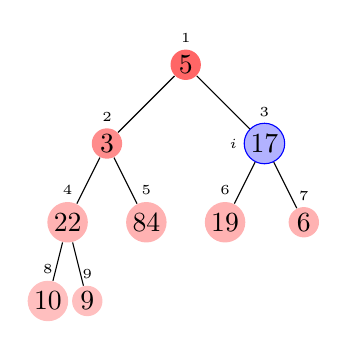
\begin{tikzpicture}
  [level distance=10mm,
    every node/.style={fill=red!60,circle,inner sep=1pt},
    level 1/.style={sibling distance=20mm,nodes={fill=red!45}},
    level 2/.style={sibling distance=10mm,nodes={fill=red!30}},
  level 3/.style={sibling distance=5mm,nodes={fill=red!25}},
]
  \node[label={90:\tiny1}] {5}
  child {node[label={90:\tiny2}] {3}
    child {node[label={90:\tiny4} ] {22}
      child {node[label={90:\tiny8}] {10}}
      child {node[label={90:\tiny9}] {9}}
    }
    child {node[label={90:\tiny5}] {84}
      child[missing] 
      child[missing]
    }
  }
  child {node[label={90:\tiny3}, label={180:\tiny$i$}, fill=blue!30, draw=blue] {17}
    child {node[label={90:\tiny6}] {19}
      child [missing]
    child [missing]
    }
    child {node[label={90:\tiny7}] {6}
        child [missing]
        child [missing]
    }
  };
\end{tikzpicture}
\end{document}





